%documentstyle{book}
\documentclass{book}

\usepackage{graphicx}

\begin{document}

\chapter{The Memory Health Approach}

A data structure may be big, but how do you know if it is too big? This chapter introduces the memory health approach, a way to gauge how efficiently a data structure uses memory. Java developers often have to piece together many smaller objects to build a single data structure. Memory health is a way to understand the overhead introduced in each object, the impact of connecting these objects into larger data structures, and, finally, how a data structure scales as it grows. Using this approach can provide valuable feedback into each step of your data modeling process.

As a programmer, you have to be concerned with both the size of your data structures and their health. Memory health is independent of size: a small structure can be unhealthy, and a large structure can be healthy. A healthy data structure will generally scale well, while unhealthy data structures are often the root causes of memory footprint problems. 

%The examples .

\section{Data or Overhead?}

The size of a data structure is the number of bytes it occupies. The \textit{health} of a data structure tells you what these bytes are accomplishing. Is the memory being spent on something important?  A very useful way to classify bytes is as either data or overhead. Bytes classified as data represent the real data intrinsic to your program. All other bytes are overhead of the particular representation you have chosen for that data. A healthy data structure, from a space standpoint, is one with a low overhead.  Sometimes there are tradeoffs; a memory bloated design may be necessary for performance. Oftentimes, with a little attention to detail, you can achieve high-performing designs with low memory overhead %(gary to fix).

Figure\ref{fig:eight-char-string} illustrates the memory costs for an eight-character Java string. You learned in the quiz in Chapter 2 that an 8-character string occupies 64 bytes, which seems surprisingly high. The actual character data takes up 16 bytes, since Java supports the international character set, which uses 2-bytes per character. So it costs 16 bytes to represent the eight characters themselves. The other 48 bytes are pure overhead. This structure has an overhead, or \emph{bloat factor}, of 75\%.   %add margin note

%add alignment
\begin{figure}
  \centering
  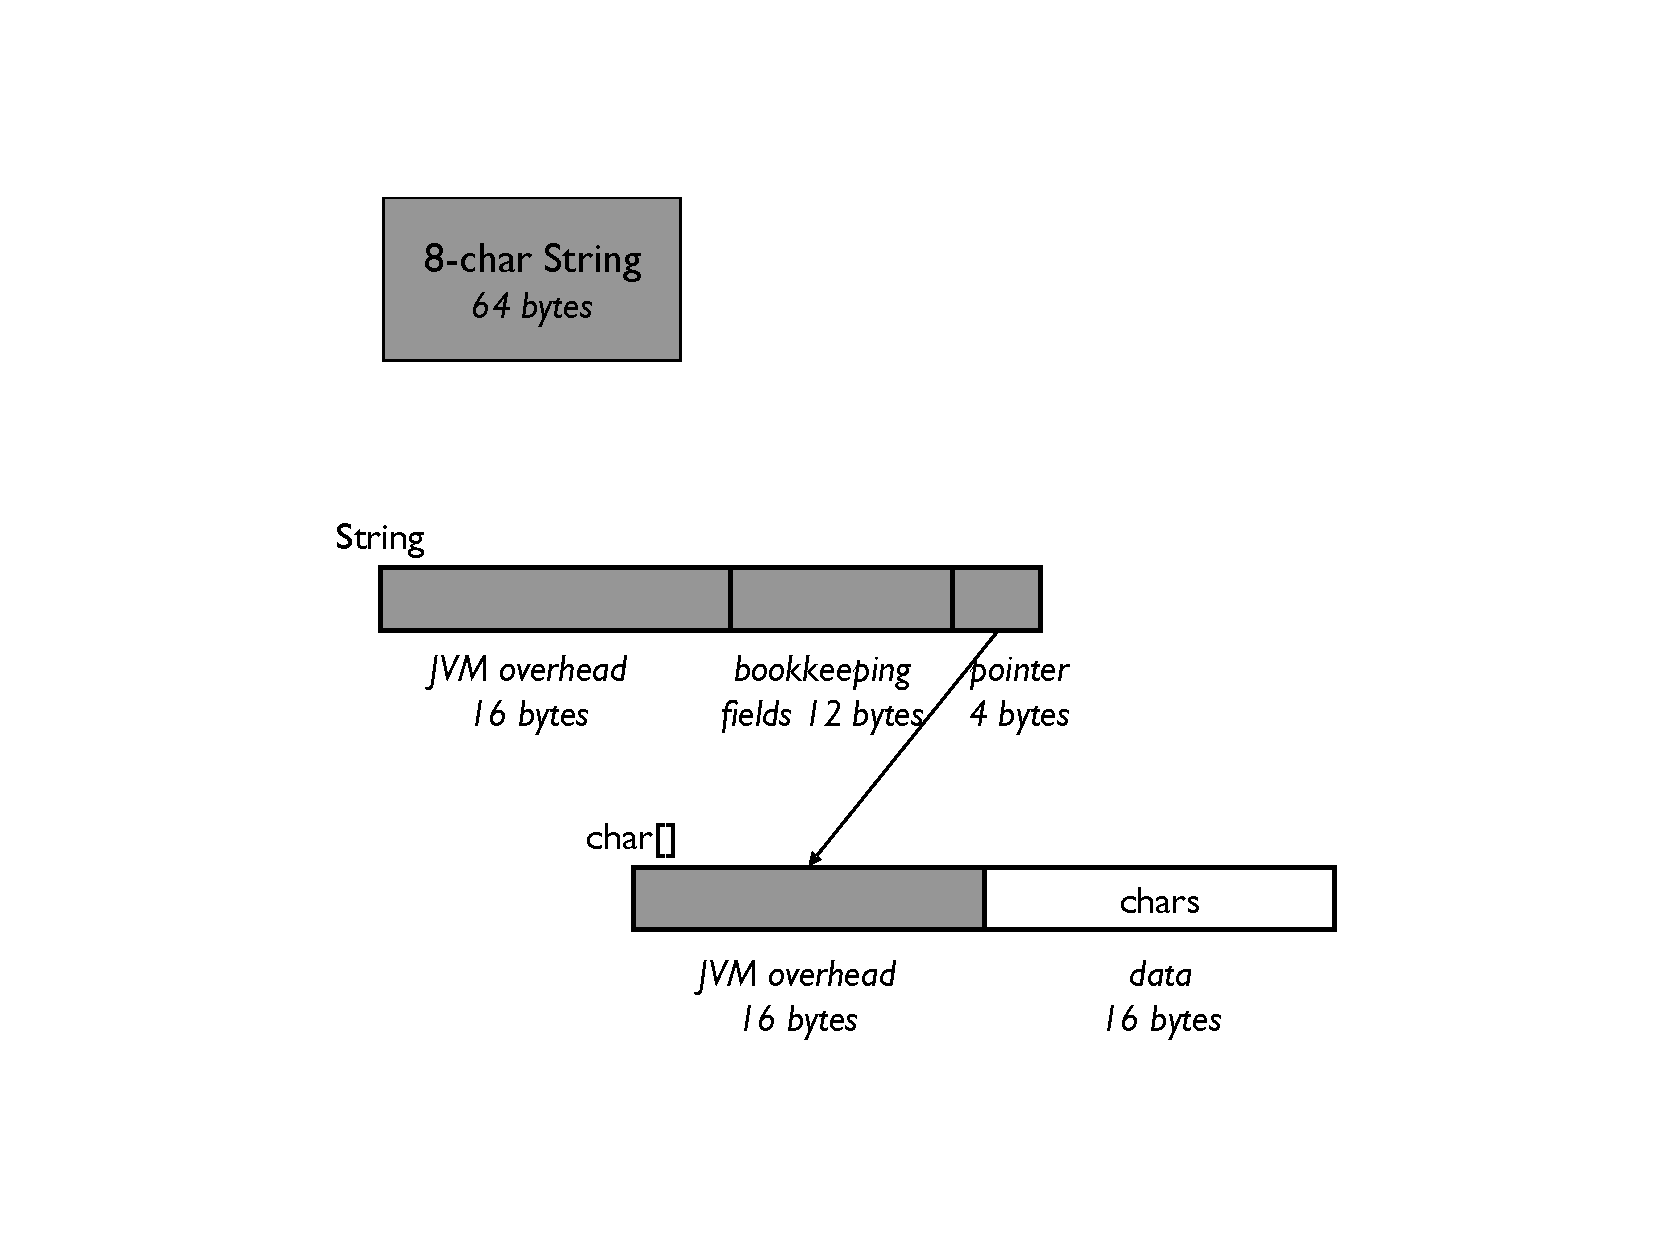
\includegraphics[width=.90\textwidth]{Figures/eight-char-string.pdf}
  %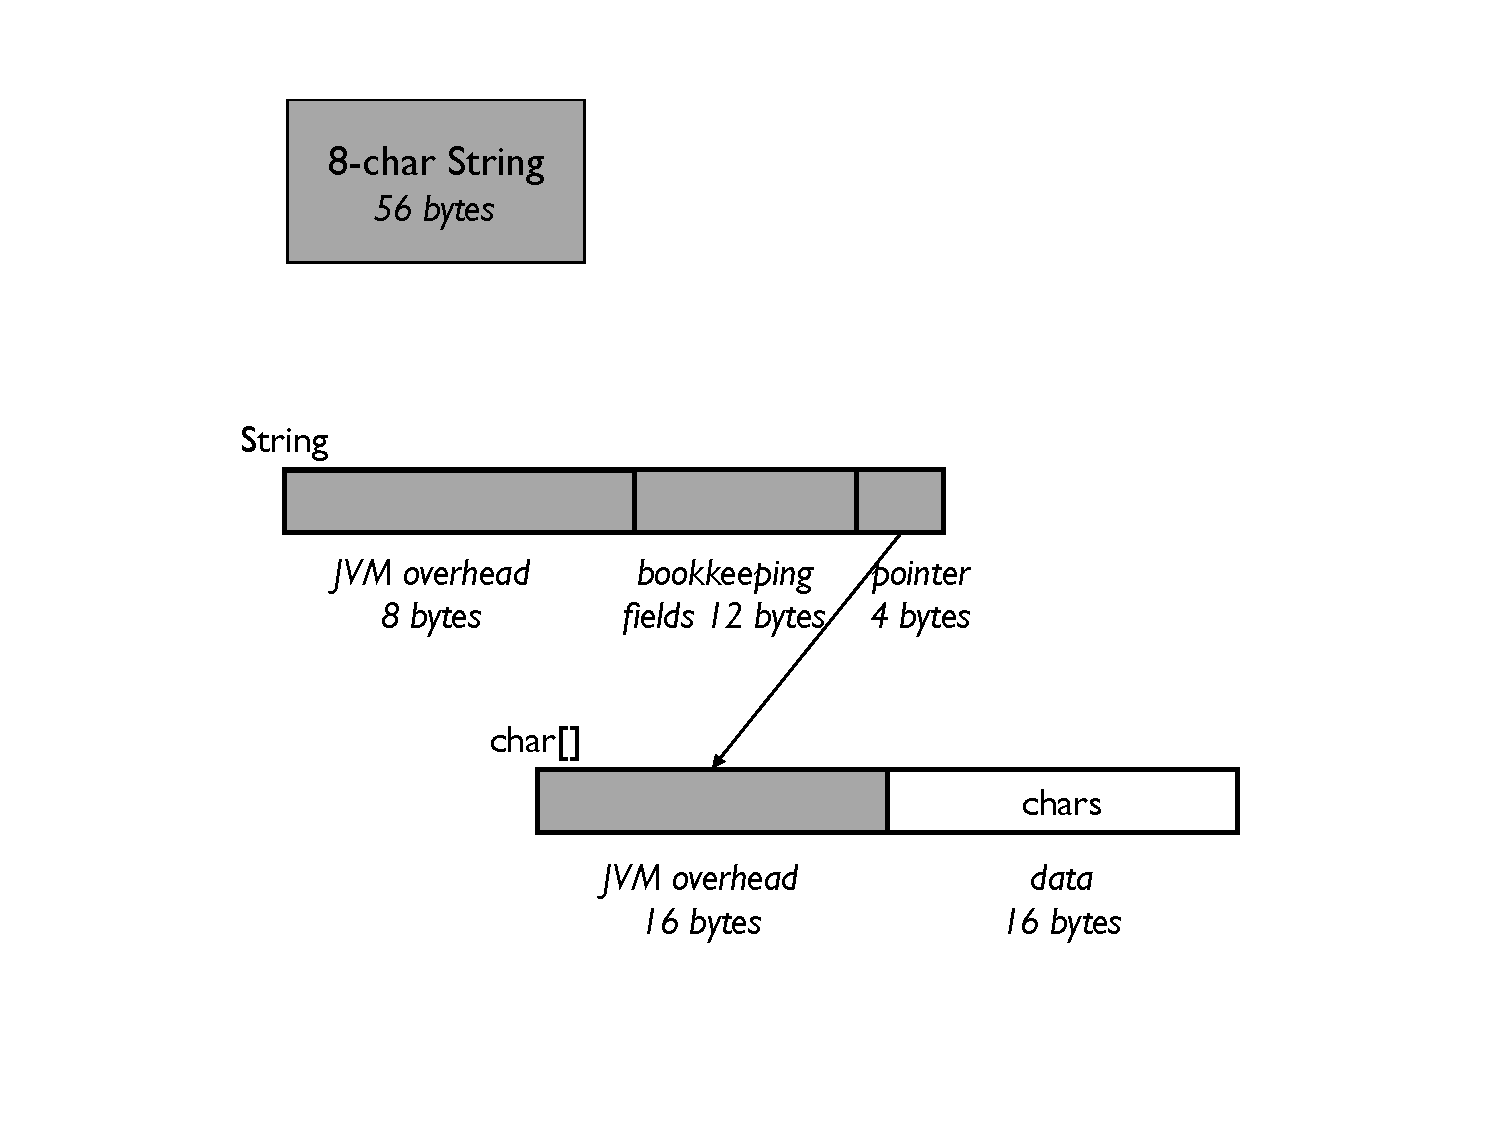
\includegraphics{eight-char-string}
  \caption{An eight character string}
  \label{fig:eight-char-string}
\end{figure}


To understand why there is so much overhead, it is useful to dig deeper into its different sources:  
\begin{itemize}
\item \textit{JVM overhead.} Each object has a header imposed by the JVM to facilitate various administrative tasks, such as garbage collection. In addition, the JVM may impose additional object alignment overhead.
\item \textit{Pointers}. Both null and non-null pointers glue objects together into data structures.   
\item \textit{Bookkeeping fields}. Not all primitive fields store real application data. Some are bookkeeping fields needed by the representation. 
\end{itemize}

Every Java string is really two objects: a {\tt String} that serves as a wrapper, and a {\tt char} array with the actual characters. Two objects means two object headers (12 bytes) and alignment costs plus a pointer gluing the two objects together. The {\tt String} object is entirely overhead, containing no real data. Part of its cost is three bookkeeping fields (12 bytes), such as a saved copy of its hashcode computation. Adding all of this together, the overhead is 48 bytes, which is 75\% of the total eight-character string. The actual data occupies only 25\%. These numbers vary depending on the particular JVM, but not significantly.\footnote{All measurements are from the 32-bit IBM Java 6 JVM.}  

If you were to design a string representation from scratch, 20\% overhead might seem a reasonable target.  The overhead cost of a string is fixed, so its relative importance shrinks for longer strings. Unfortunately, for a string to have only 20\% overhead, it would need to be 96 characters long. As bad as this seems, for some data structures it is not even possible to amortize away overhead costs, as discussed in Section~\ref{scalability}.  

\texttt{String}s, in particular short strings, are pervasive. It is important to be aware of the overhead of strings when incorporating them into your data design. Given the overhead of strings in Java, the choices you make in Java need to be different than in a language like C, where the string overhead is minimal. Making informed choices is critical for the overall memory health of an application. There will be more on strings in later chapters.

\section{Data Structure Cost Notation}

It is useful to have a diagram notation to illustrate more complex examples, as a way of talking about a data structure and how it uses memory. Figure~\ref{fig:content-schematic} shows the basic elements of a \textit{content schematic}. A content schematic summarizes the cost breakdown of a data structure.

\begin{figure}
  \centering
  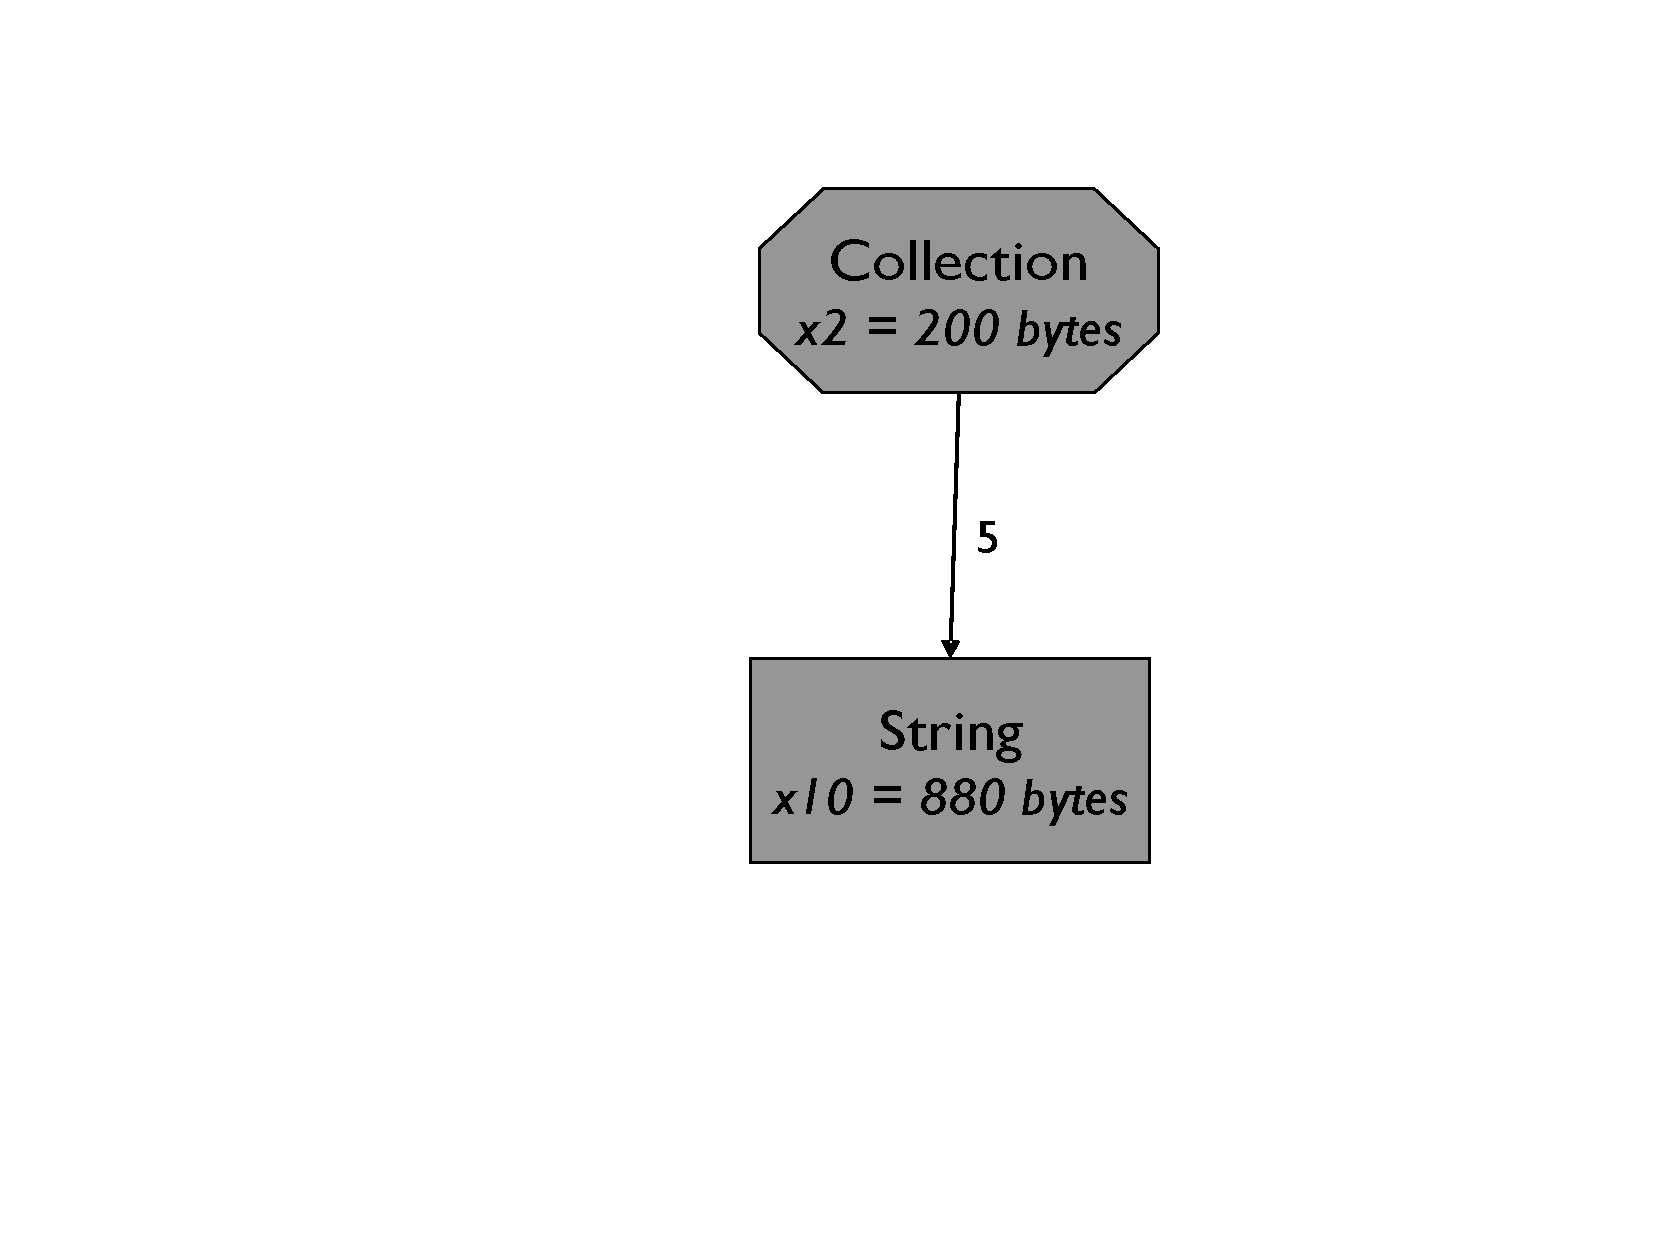
\includegraphics[width=0.9\textwidth]{Figures/content-schematic}
  \caption{A content schematic}
  \label{fig:content-schematic}
\end{figure}
	
There are two types of boxes, or entities, in a content schematic. Octagons represent collection infrastructure, and rectangles represent all other entities. An edge from a collection to a rectangular entity indicates membership of the entity in the collection. The notation \textit{xN }inside each entity means there are \textit{N} instances of the entity. The expression \textit{xN = M} bytes means that there are \textit{N} instances occupying \textit{M} bytes of memory. An edge in a content schematic is labeled with the average fanout from the source entity to the target entity.

In Figure~\ref{fig:content-schematic}, there are two \texttt{Collection}s which together occupy 200 bytes, and ten \texttt{String}s occupy 880 bytes. There are on average five elements contained in each of the two \texttt{Collection}. Since the overhead of a \texttt{String} is 48 bytes and there are 10 \texttt{String}s, the total overhead is 480 bytes or 55\%. Data occupies 400 bytes, so the average \texttt{String} length is 10. The two \texttt{Collection}s are pure overhead, so the total overhead of this data structure is 680 bytes, or 63\%.
	
The entities in a content schematic are abstracted from the actual data structure objects. A box may be hiding other objects that help implement the entity. For example, the \texttt{String} entity in Figure~\ref{fig:content-schematic} represents both \texttt{String} and \texttt{char} array objects. The name of an entity is the name of the top object. Entities also summarize objects of the same type that are repeated in a data structure.  The \texttt{String} entity in Figure~\ref{fig:content-schematic} represents the 10 \texttt{String}s in the two \texttt{Collection}s. The memory cost of an entity is the sum over all of its objects. This summarization removes clutter and helps understanding. 

Content schematics are a little like UML diagrams, since they represent a schematic of entities and relationships. Unlike UML diagrams, relationships are elevated to be entities, rather than edges. The reason is that in a language like Java, implementation of the relationship itself is often a big cause of expense, so it is important to make that visible. A very common pattern is to implement relationships as collections. Figure~\ref{fig:content-schematic-relationship} shows a map from 10K \texttt{Strings} to 10K \texttt{Doubles}, which is implemented by a \texttt{HashMap}. You can compute the memory health as an exercise.
  
\begin{figure}
  \centering
  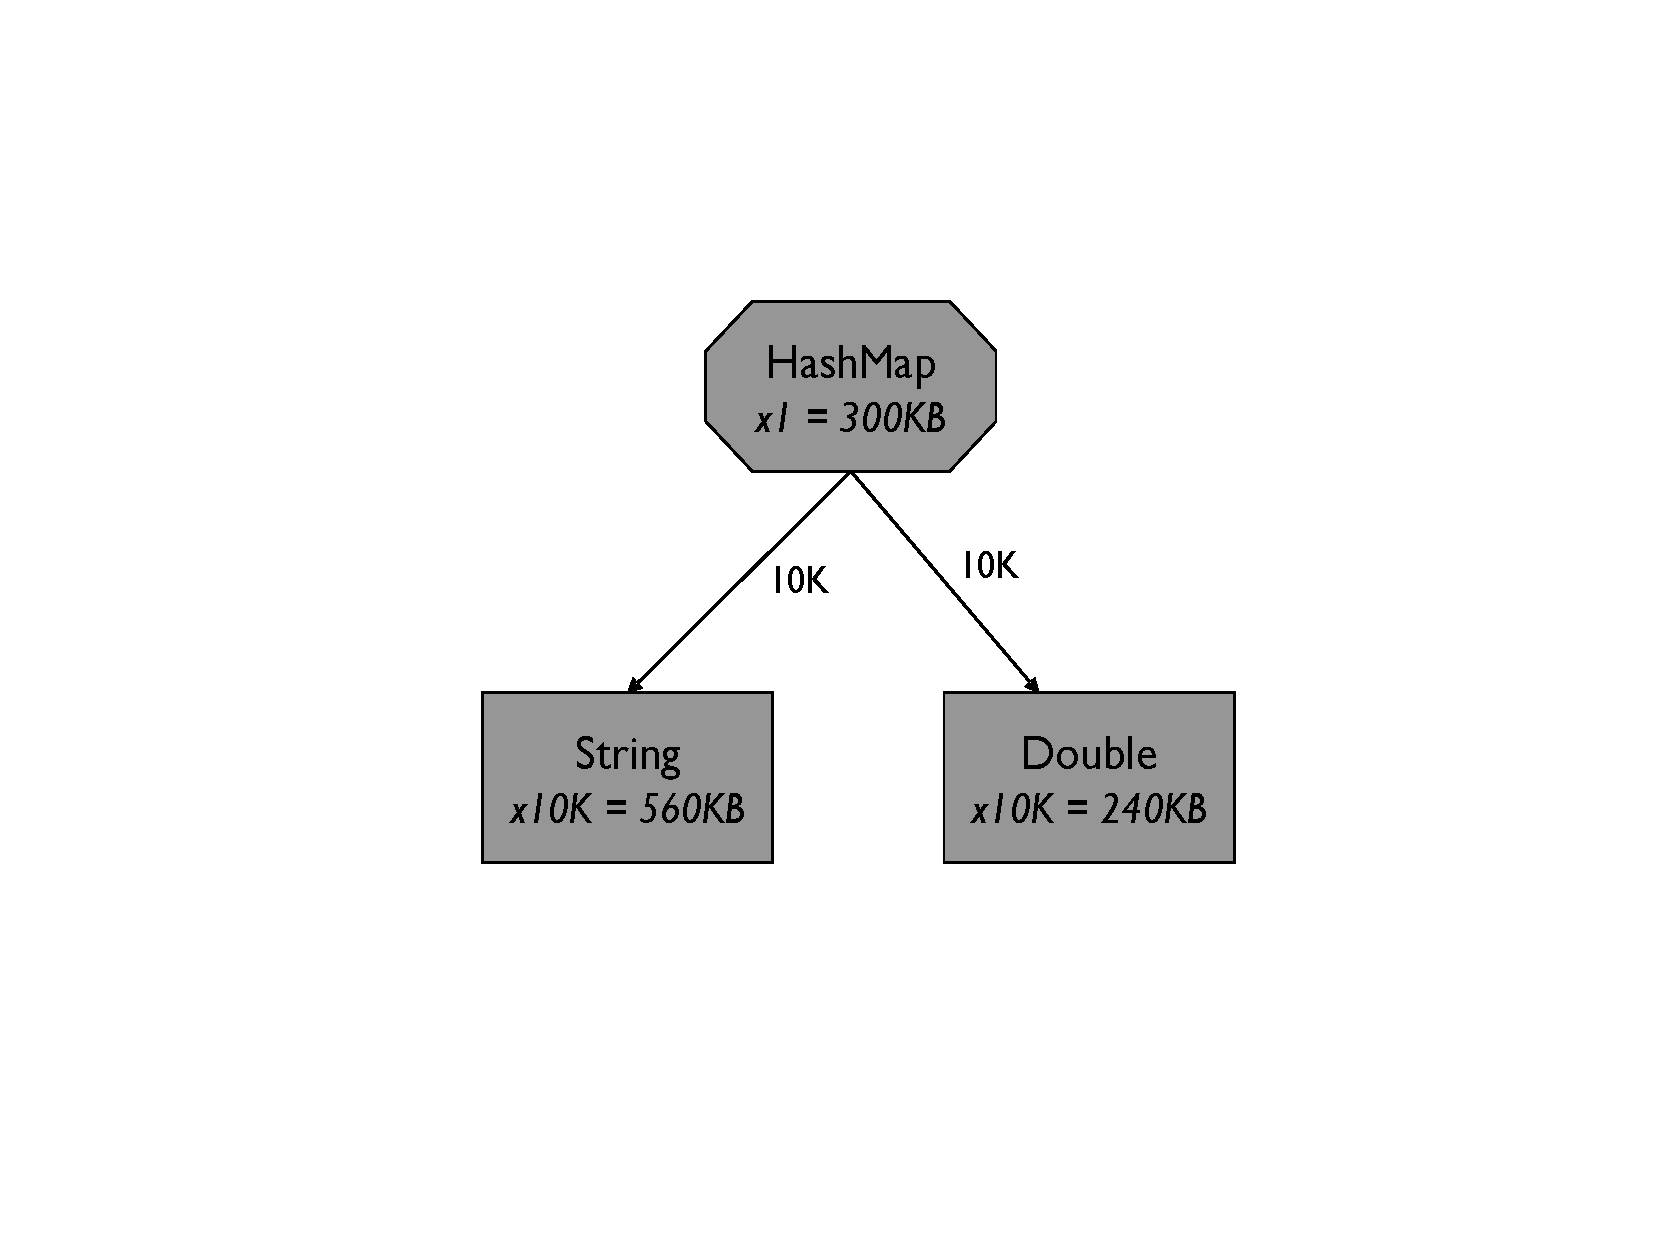
\includegraphics[width=0.9\textwidth]{Figures/content-schematic-relationship}
  \caption{A content schematic of a map from 10K \texttt{Strings} to 10K \texttt{Doubles}.}
  \label{fig:content-schematic-relationship}
\end{figure}


\section{Example: Sorted Map of Doubles}
\label{section:mapofdoubles}

Consider the following problem. The first phase of a program needs to read in a map of doubles to doubles, so that a second program phase can retrieve the map entries in sorted order by key. The details of this second phase are not important here. This scenario is an example of a very common more general pattern:
 
\textit{Load-and-Use Behavior Pattern:} load data in one phase, use the data in the next phase.
 
The problem is to design a data structure to store this map of doubles. A regular \texttt{HashMap} is not a good choice here, since it is not possible to keep the map entries sorted in a \textit{HashMap}. This section describes are three designs for a map of doubles with 100 entries. These designs have vastly different memory health characteristics. For each of these designs, the amount of actual data is the same. A double is eight bytes, each entry has two doubles, so 100 entries occupies 1.6KB. The difference is in the overhead.

\textbf{Solution 1.} The first idea that leaps forward is to use a \texttt{TreeMap}. Conveniently, the Java \texttt{TreeMap} class is a map that maintains its entries in sorted order, so this appears to be a perfect choice. The only problem is the memory cost.

A content schematic for a 100-entry map of doubles using TreeMap is shown in Figure~\ref{fig:content-schematic-treemap-doubles}.  The total cost of this data structure is 8.5KB. Since there is only 1.6KB of data, the overhead is 7KB, which is 82\%. What is costing so much?

\begin{figure}
  \centering
  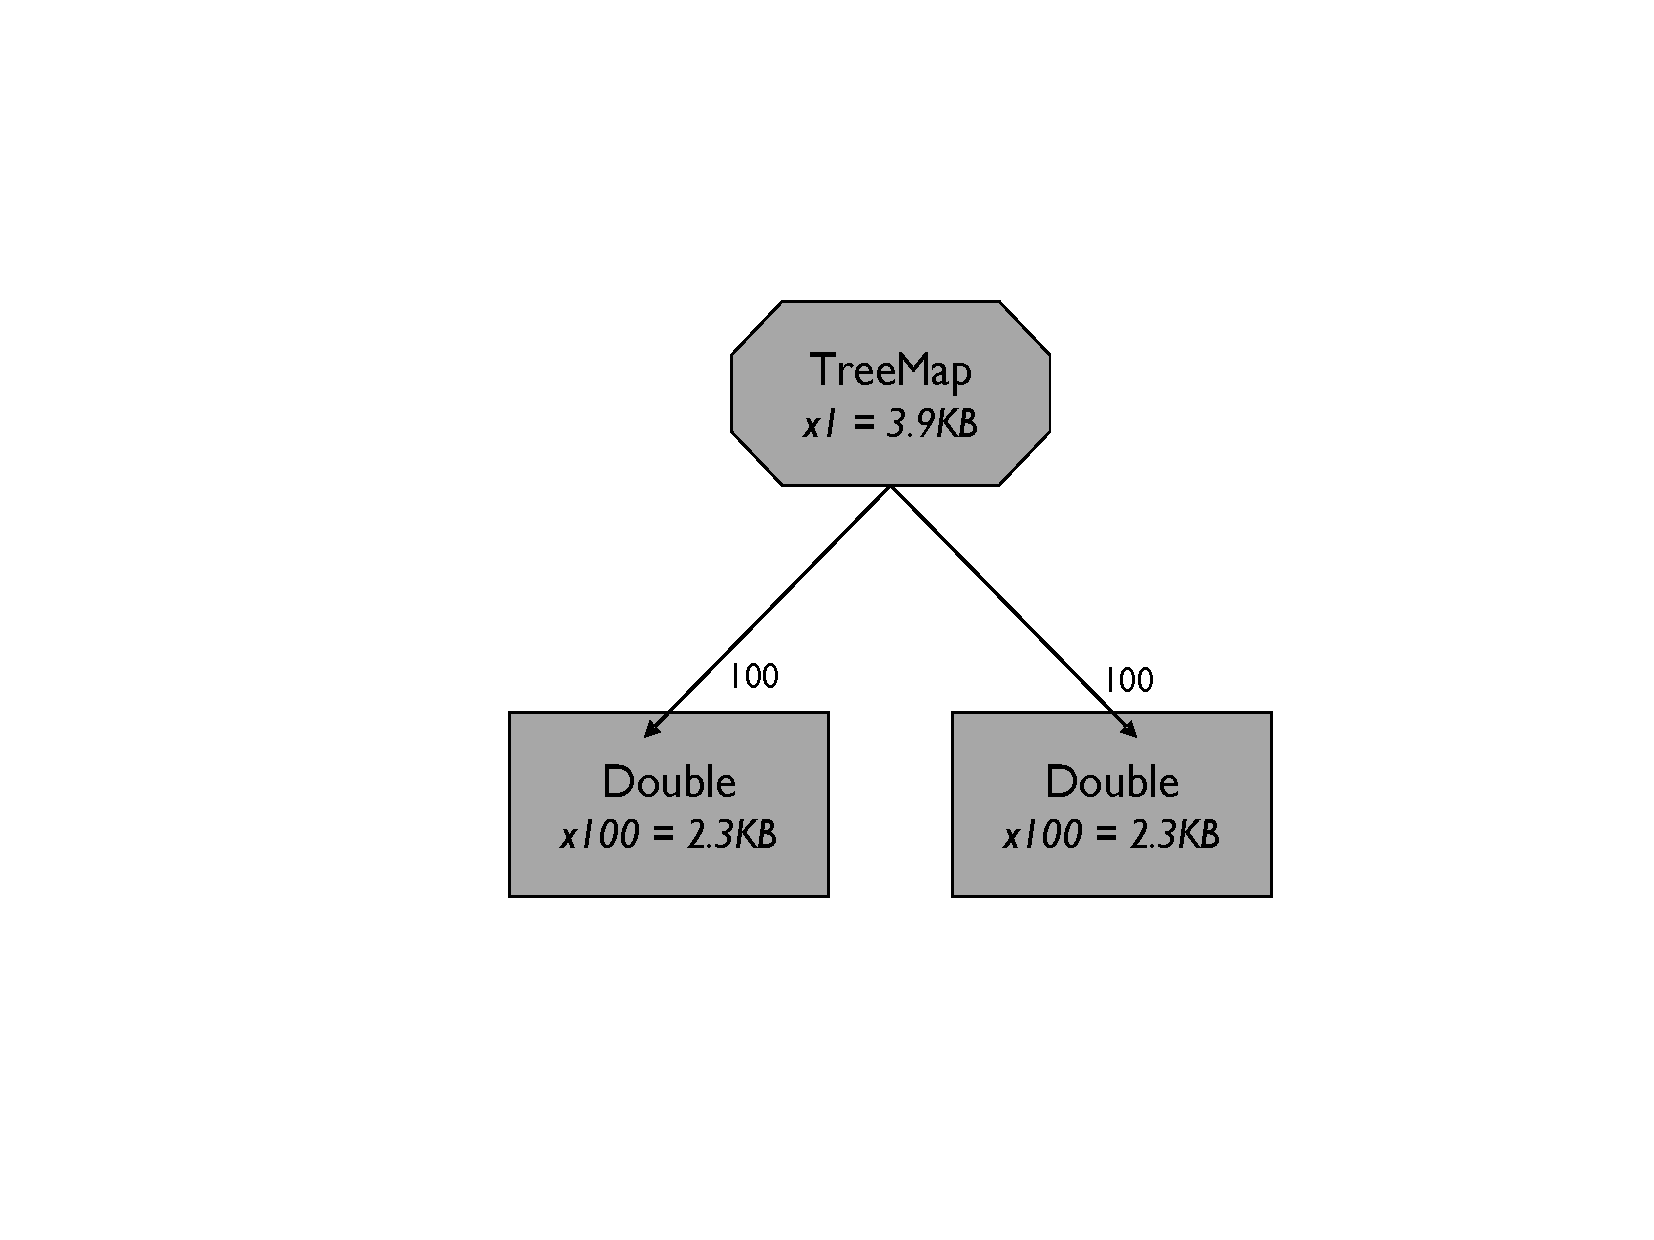
\includegraphics[width=0.9\textwidth]{Figures/content-schematic-treemap-doubles}
  \caption{Solution 1: \texttt{TreeMap} of \texttt{Doubles}}
  \label{fig:content-schematic-treemap-doubles}
\end{figure} 
 
Looking inside the individual entities can provide some insight. First, the doubles themselves are stored in \texttt{Double} objects, since scalars must be boxed before storing them in a standard Java collection.  A single instance of a \texttt{Double} object is 24 bytes. Since the data is only 8 bytes,  33\% of a \texttt{Double} object is actual data, and 67\% overhead. This is a high price for a basic data type. At best, the overhead will be 67\% if the doubles are boxed.

The next surprise is that while there are 200 \texttt{Doubles}, there is only one \texttt{TreeMap}, but it is consuming a whopping 3.9KB of memory. All of this is overhead. What is taking up so much space in there? A \texttt{TreeMap}, like every other collection in Java, has some kind of wrapper object, the \texttt{TreeMap} object itself, and, in this case, it points to 100 \texttt{TreeMap\$Entry} objects. Each type of collection in the standard library has a different kind of infrastructure, some point to arrays, some point to separate entry objects. In the case of \texttt{TreeMap}, for each entry, there is a separate \texttt{Treemap\$Entry} object. This is typical of collections. A typical collection has a fixed overhead, in this case it is 48 bytes, and a per-entry overhead cost, in this case it is 40 bytes per entry. These 40 bytes include five pointer fields, in addition to other sources of overhead. This relatively high per-entry cost makes \texttt{TreeMap} a particularly expensive collection. The costs of other collections are given in Chapter 7.
 
Using a \texttt{TreeMap} is not necessarily a wrong design. It depends on whether that 82\% overhead is buying something useful. In this example, the main thing it is buying is the ability of \texttt{TreeMap} to maintain a sorted order while randomly inserting and deleting elements. It constantly maintains a sorted order. If you need something to be in sorted order during the load phase, or maybe you have a real time monitor that is constantly being updated, and you need to look at it in that order, then \texttt{TreeMap} is a great data structure.  But if you do not need this functionality, there are other data structures that could accomplish the same thing more cheaply. In this example, the sorted order is only needed during the second phase, after all the data is loaded. The load-and-use behavior can be exploited to choose a cheaper representation.

Of course, the other nice thing about \texttt{TreeMap} is that it can be pulled off the shelf. But maybe there are other collection classes that are available, or maybe there are other kinds of collection classes that can be put together. This does not mean that programmers should be writing their own collections, but there are some cases where you can slap a thin wrapper over something that already exists.

\textbf{Solution 2.} This next design uses a more efficient data structure than \texttt{TreeMap}. The sorted order is not maintained when the data is being loaded, but this is not a problem. This design stores the double map in an \texttt{ArrayList}, where each entry is a pair of doubles. There is a bit more programming required to implement this solution, but it is not excessive. Fortunately, the Java standard \texttt{Collections} class has some useful static methods, namely, a \texttt{sort} method and a \texttt{binarySearch} method. Each of these can take an \texttt{ArrayList} and a \texttt{Comparator} as parameters. This design requires writing two new classes:

\ttfamily
\begin{verbatim}
   
    public class Pair {

        private double key;
        private double value;
	
        public Pair(double d1, double d2) {
            key = d1;
            value = d2;
        }
	
        public double getKey() {
            return key;
        }
	
        public double getValue() {
            return value;
	      }
    }

   
    public class ComparePairs implements java.util.Comparator<Pair>  {
    
        public int compare(Pair p1, Pair p2){
		
            double d1 = p1.getKey();
            double d2 = p2.getKey();
			
            if (d1 < d2) {
                return -1;
            } else if (d1 == d2) {
                return 0;
            }
            return 1;
        }
    }
\end{verbatim}
\normalfont

Additionally, there needs to be a wrapper class, to implement map operations. This wrapper can either implement the Java \texttt{Map} interface, or something similar. Here is a skeleton showing the \texttt{get} method for this wrapper class:

\ttfamily
\begin{verbatim}
    public class DoubleMap implements java.util.Map {

        private ArrayList<Pair> ar = new ArrayList<Pair>();
        static ComparePairs comparator = new ComparePairs();
        ....
		
        /* Parameter O is a Double, returns Double */
        public Object get(Object O) {
            Pair p = new Pair(((Double) O).doubleValue(), 0.0);
            int result = Collections.binarySearch(ar, p, comparator);
            if (result < 0) return null;
            return new Double(ar.get(result).getValue());
        }
		
        public void sort() {
            Collections.sort(ar, comparator);	
        }
    }
    
\end{verbatim}
\normalfont   

The content schematic for 100 entries is shown 
in Figure~\ref{fig:content-schematic-arraylist-pairs}.
\begin{figure}
  \centering
 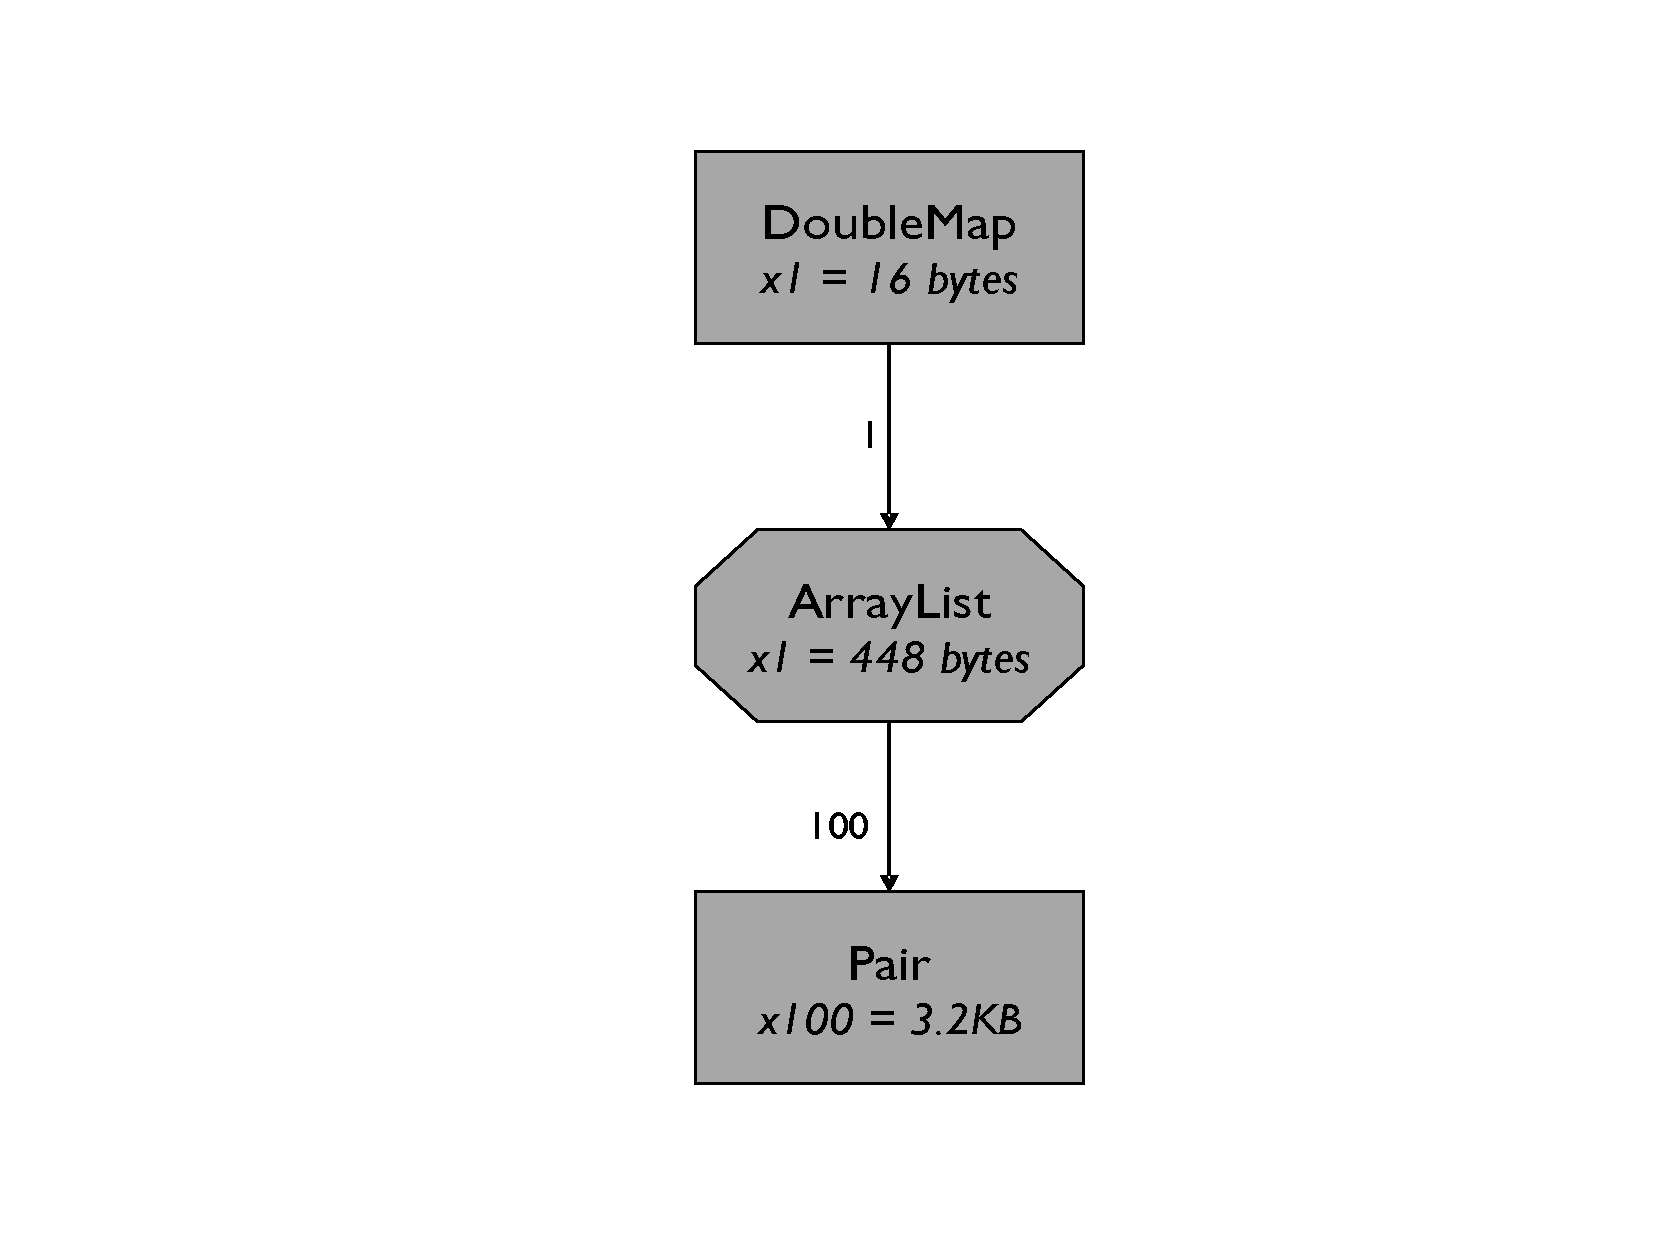
\includegraphics[width=0.9\textwidth]{Figures/content-schematic-arraylist-doubles}
  \caption{A content schematic for an \texttt{ArrayList} of \texttt{Pairs}}
  \label{fig:content-schematic-arraylist-doubles}
\end{figure} 

This solution is cheaper than the \texttt{TreeMap} solution for two reasons. First, the doubles are not boxed. The 100 entries requires only 100 \texttt{Pair} objects. The \texttt{TreeMap} solution requires 200 objects to store all of the keys and values as boxed \texttt{Doubles}. This means that there are at least 100 fewer object headers in the \texttt{ArrayList} solution. Secondly, the per-entry cost of an \texttt{ArrayList} is much smaller than the per-entry cost of a \texttt{TreeMap}. Instead of 40 bytes per entry, the cost is 4 bytes per entry for an \texttt{ArrayList}. This is because an \texttt{ArrayList}, not surprisingly, stores its entries in an array. The incremental cost of an entry is a single pointer. 

\textbf{Solution 3.} This last alternative is an optimal, no-overhead solution. Eliminating overhead requires eliminating objects altogether. This is not a recommended practice, unless memory is extremely tight, and there is no other choice. It is none the less interesting to compare this best case solution with the others. It uses two parallel arrays of doubles. One array stores all of the keys, and the second stores all of the values. You need to encapsulate these arrays in a wrapper object, to provide an object fa�ade.

In addition to forsaking objects, this design requires a bit more code, but, again, it is not excessive. Like the \texttt{Collections} class, The Java \texttt{Arrays} class has \texttt{sort} and  \texttt{binarySearch} methods that can be pulled off the shelf. However, these methods apply only to a single array. If you sort the keys, you lose the association between the keys and their corresponding values. You can use an extra temporary array to get around this problem. The solution is left as an exercise.
 
The context schematic for two arrays of 100 doubles is shown in 
Figure~\ref{fig:content-schematic-arrays-doubles}.  The overhead consists of two object headers, which is 2\% of the total structure (probably more with the wrapper -- add).

\begin{figure}
  \centering
  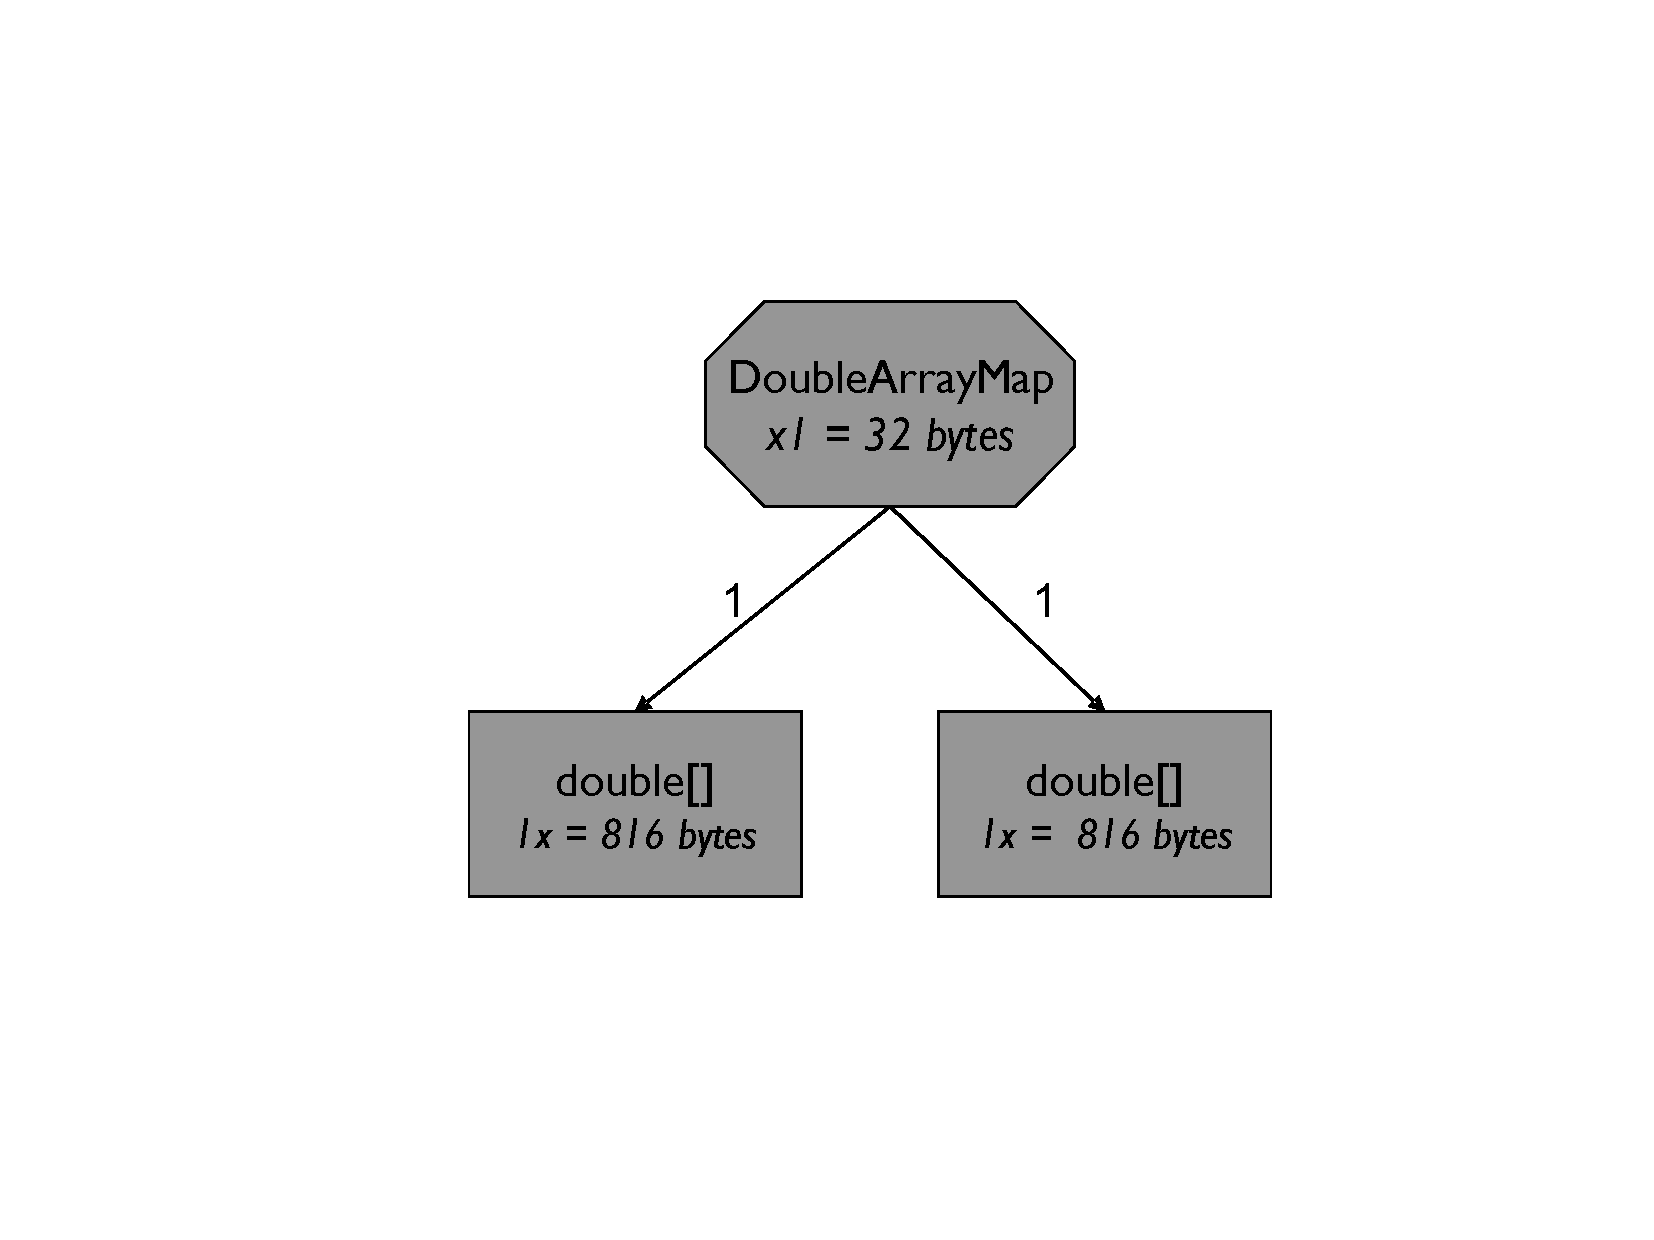
\includegraphics[width=0.9\textwidth]{Figures/content-schematic-arrays-doubles}
  \caption{Content Schematic for arrays of \texttt{doubles}}
  \label{fig:content-schematic-arrays-doubles}
\end{figure}

Another option is to use one data structure in the first phase, and copy it into a second data structure for the second phase. For example, the \texttt{ArrayList} solution could be used for the first phase, and the \texttt{double} array solution for the second phase.

In this example, there is a tradeoff between ease of programming and memory efficiency. More code is needed for solution 2, and even more code for solution 3. However, in many cases, memory efficient designs are just as easy to implement as inefficient designs.
 
\section{Scalability}
\label{scalability}

The example in Section~\ref{section:mapofdoubles} deals with a relatively small amount of data.  There are only 100 entries in the map of doubles.  Maybe if the solution is scaled up to say 10,000 entries, the high cost of the first \texttt{TreeMap} solution will be amortized away, and you will be just fine. Unfortunately, a 10,000 entry \texttt{TreeMap} is still at 82\% overhead. The reason here is that the overhead costs are per entry costs, and they are high.  So whenever you add an entry, this adds two \texttt{Doubles}, with all their boxing costs, and a 40 byte \texttt{TreeMap\$Entry} object. Each entry costs 88 bytes, and only 18\% of that cost is actual data. So in effect, this design  is not only bloated, but it also does not scale. It is constantly bloated. 
\begin{figure}
  \centering
  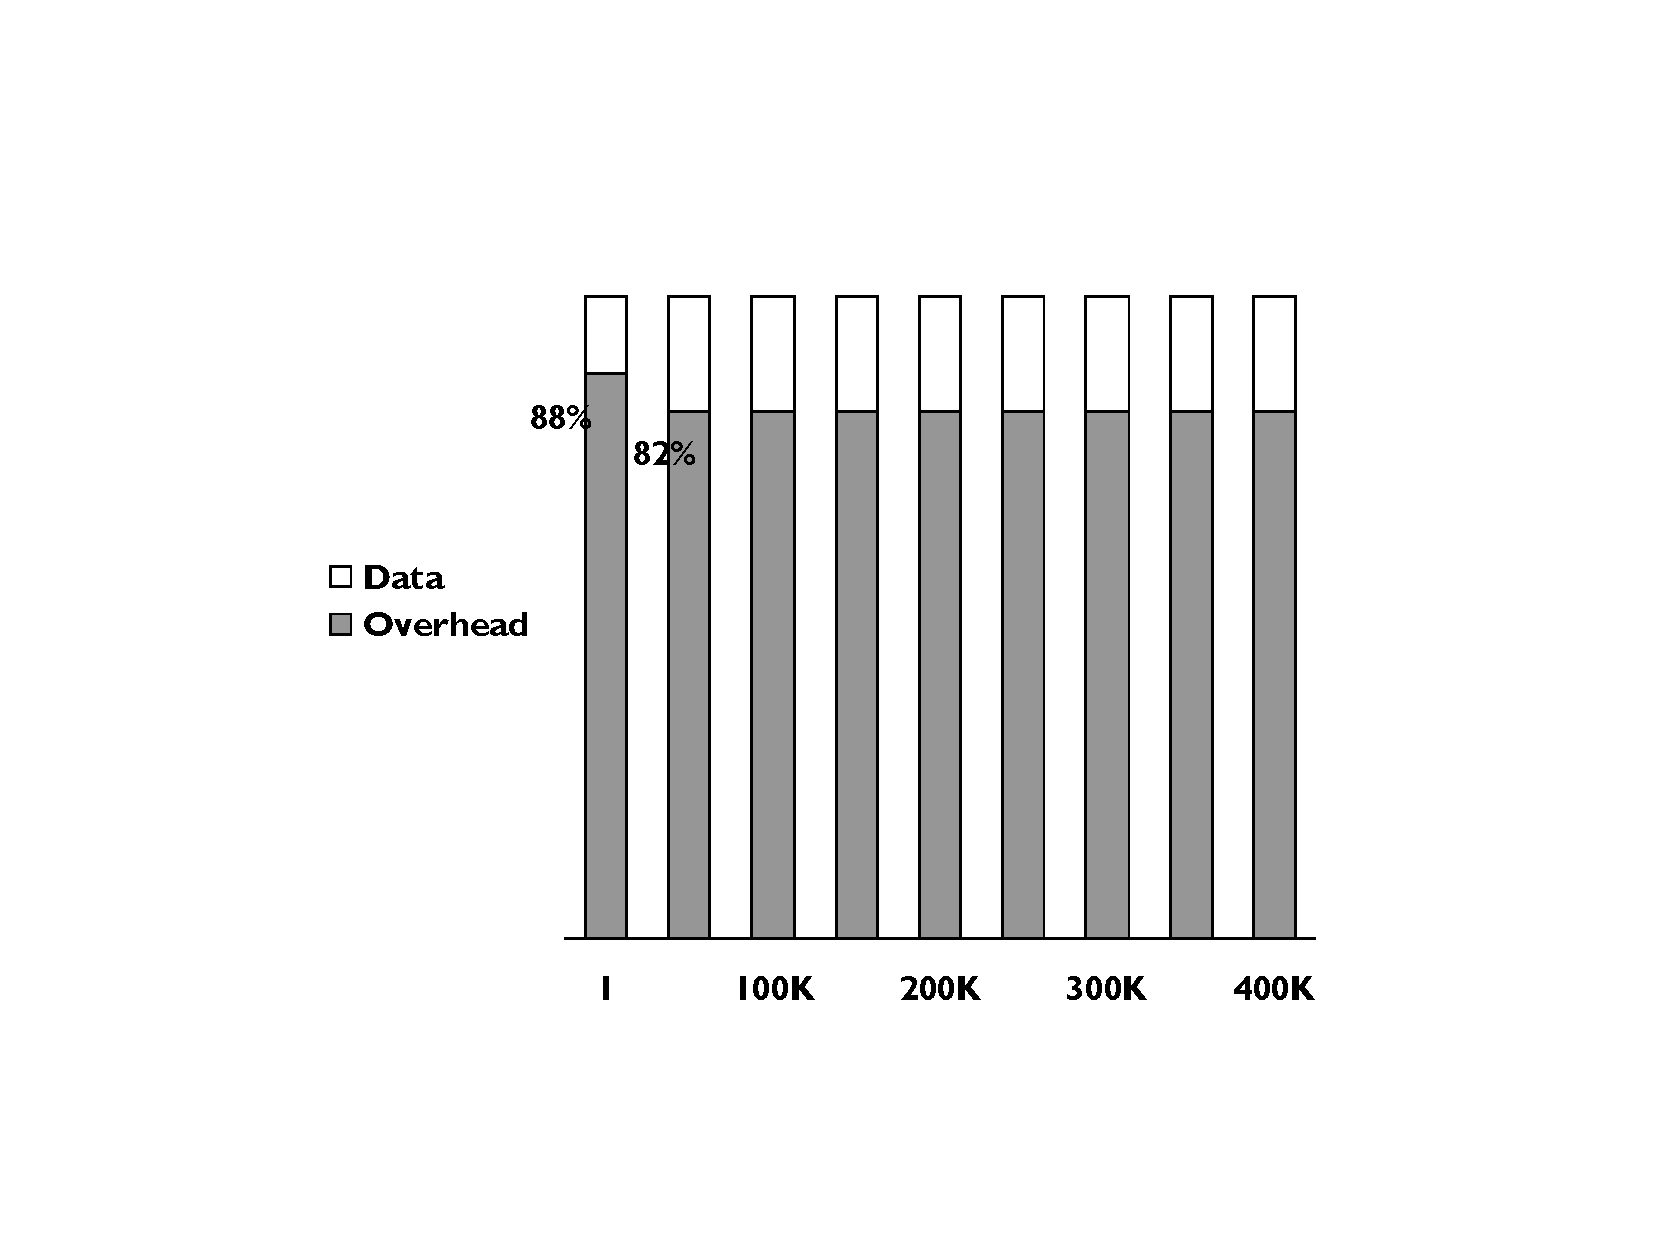
\includegraphics[width=0.9\textwidth]{Figures/scalable-health-treemap}
  \caption{Health Measure for TreeMap Solution Shows Poor Scalability}
  \label{fig:scalable-health-treemap}
\end{figure}

\begin{figure}
  \centering
  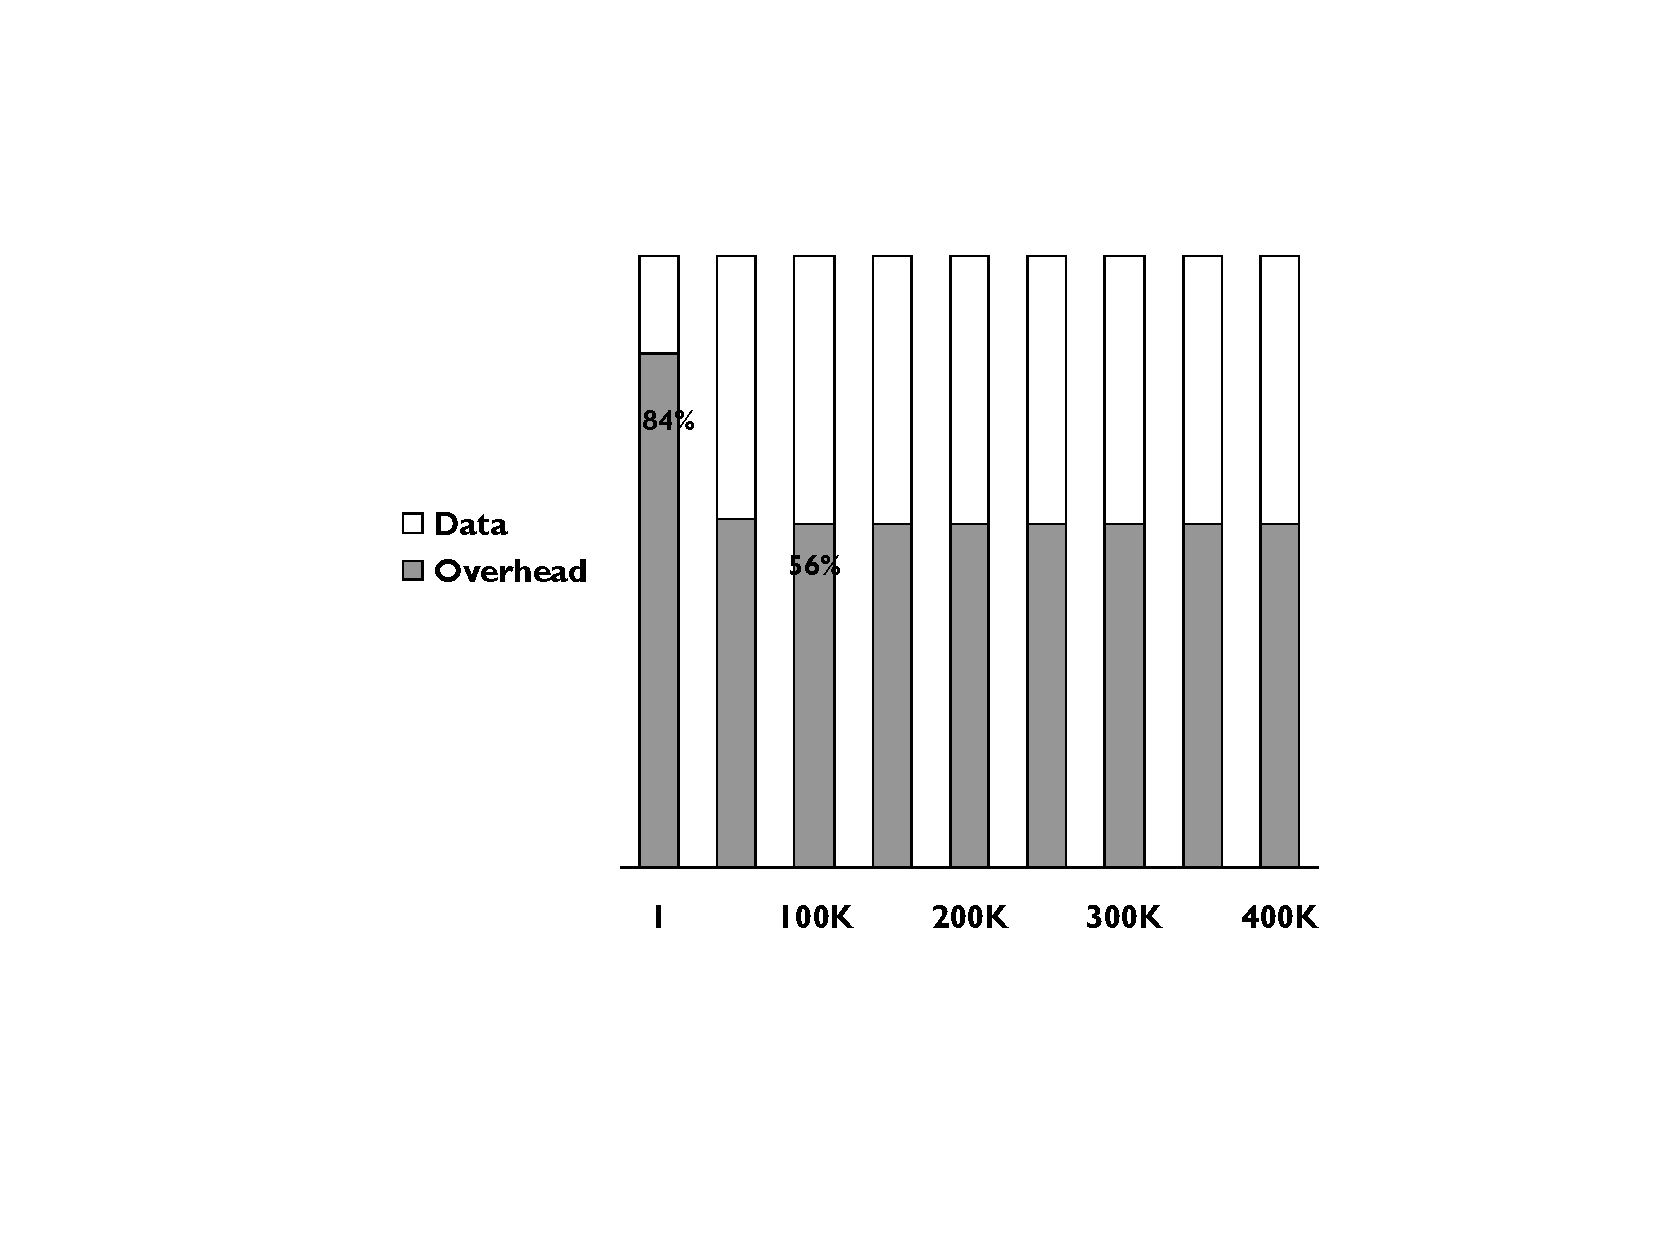
\includegraphics[width=0.9\textwidth]{Figures/scalable-health-arraylist}
  \caption{Health Measure for ArrayList Solution Shows Good Scalability}
  \label{fig:scalable-health-arraylist}
\end{figure}

The memory health concept can be used to gauge scalability, which parts of our design are scalable and which parts are not scalable. The bar graph in Figure~\ref{fig:scalable-health-treemap} shows how the \texttt{TreeMap} solution from Section ~\ref{section:mapofdoubles} scales as the number of entries increase. Each bar is split into two parts: the percentage of overhead and the percentage of data.  When there are only a few entries, the overhead is 88\%, since the fixed cost of the \texttt{TreeMap} is significant. Very quickly this fixed cost is amortized away. After that, there is a constant per entry overhead of 82\%. With this information, it is possible to predict how much memory a data structure will occupy for a given input size. For a map with 1M entries, the overhead would be 89MB, and the total cost would be 105MB.

With the two \texttt{double} array design, there is only fixed overhead, a container object and two object headers, which is 4\% for 100 entries, as shown in Figure~\ref{fig:scalable-health-array}. Once the fixed cost is amortized, which happens quickly, the overhead goes down to 0. You really are just paying for pure data here.

\begin{figure}
  \centering
  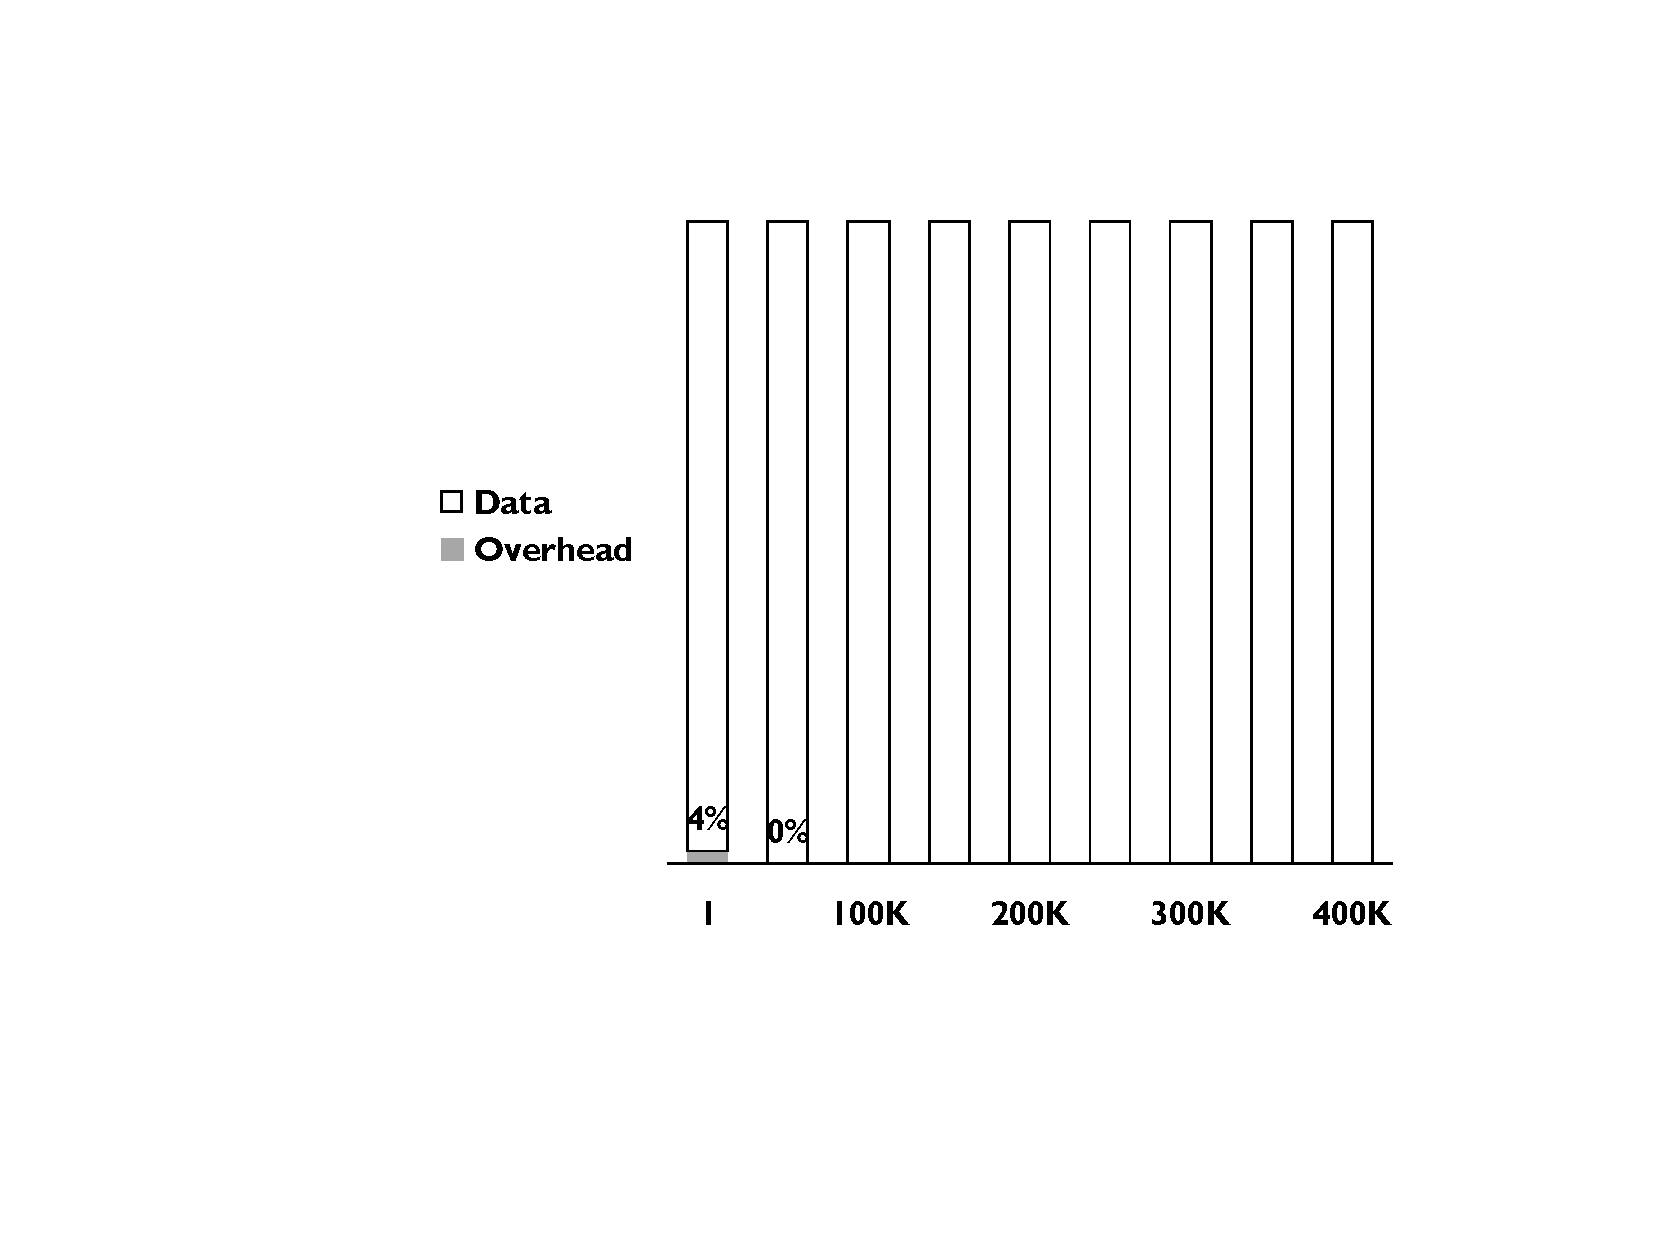
\includegraphics[width=0.9\textwidth]{Figures/scalable-health-array}
  \caption{Health Measure for Array Solution Shows Perfect Scalability}
  \label{fig:scalable-health-array}
\end{figure}

Knowledge of data structure scalability is very valuable early in the design process. Too often, performance problems are addressed late in the process, when they are much harder to address. By measuring the memory health of your design early on, and understanding its scalability, you can avoid costly redesigns later on.  


\section{Summary}

This chapter introduced the concept of memory health as a way thinking about the memory efficiency of a data design. How much of your design is real data, and how much is an artifact of the way you are representing it. The answer will show you how much room for improvement there is, and if in fact you are paying a reasonable price for what you are getting.

Memory health is defined here simply as low overhead cost. Each byte is classified as data or overhead. 
You can define more sophisticated health metrics. There are different kinds of overhead, and you can dissect and measure it in a variety of ways. For example, you can measure empty array slots or different classes of pointers. Memory health is treated more formally in [reference paper].


When you are developing a large application, closing your eyes to quantitative considerations and thinking everything is going to be fine is not a good option. Nevertheless, you should not throw out all the Java libraries and write everything yourself. Taking the time to measure the cost and health of your data design can pinpoint problems early on. It can also prevent unnecessary optimizations that gain little or nothing. You should perform thought experiments, use limit cases to understand optimal designs, and make back-of-the-envelope calculations.  This requires more work, possibly more prototyping, but the effort will likely pays off. Subsequent chapters discuss more techniques for precise estimation of memory health, and provide the data and overhead costs of common primitives and collections needed to perform estimations. 


\end{document}
